
\subsection*{Partie A}

Le discriminant de \( P(x) = -10x^2 - 40x + 120 \) est donné par :
\[
\Delta = (-40)^2 - 4 \times (-10) \times 120 = 1600 + 4800 = 6400 = 80^2.
\]
Ce polynôme a deux racines réelles distinctes :
\[
x_1 = \frac{40 - 80}{-20} = 2 \quad \text{et} \quad x_2 = \frac{40 + 80}{-20} = -6.
\]

\( P(x) = 0 \) pour \( x = -6 \) et \( x = 2 \).

Le coefficient du terme en \( x^2 \) est négatif, ce qui indique que \( P(x) < 0 \) sauf sur l'intervalle \( ]-6\,;\,2[ \) où \( P(x) > 0 \).

\subsection*{Partie B}

L'aire du rectangle ABDE est donnée par :
\begin{align*}
\mathcal{A}_{ABDE} &= AB \times AE \\
&= (8 - x)\left( \dfrac{10x + 4}{x + 2} - 0 \right) \\
&= \dfrac{(8 - x)(10x + 4)}{x + 2}
\end{align*}

\paragraph{1.} Lorsque \( x = 0 \) :
\[
\mathcal{A}_{ABDE} = \dfrac{(8 - 0)(10 \times 0 + 4)}{0 + 2} = \frac{32}{2} = 16,
\]
donc de 16 unités d'aire.

\paragraph{2.} Lorsque \( x = 4 \) :
\[
\mathcal{A}_{ABDE} = \dfrac{(8 - 4)(10 \times 4 + 4)}{4 + 2} = \frac{176}{6} \approx 29{,}33,
\]
donc environ de 29{,}33 unités d'aire.

\paragraph{3.}

\begin{align*}
f'(x) &= \frac{(-20x + 76)(x + 2) - (-10x^2 + 76x + 32) \times 1}{(x + 2)^2} \\
&= \frac{-20x^2 + 36x + 152 - (-10x^2 + 76x + 32)}{(x + 2)^2} \\
&= \frac{-10x^2 - 40x + 120}{(x + 2)^2}.
\end{align*}
On déduit de la partie A :
\begin{center}
\begin{tikzpicture}
\tkzTabInit[lgt=4, espcl=3.5]{$x$ / 1, {$(x + 2)^2$} / 1, {$-10x^2 - 40x + 120$} / 1, {Signe de $f'(x)$} / 1, {$f$} / 2}{${0}$, ${2}$, ${8}$}
\tkzTabLine{,+,,+,}
\tkzTabLine{,+,0,-,}
\tkzTabLine{,+,0,-,}
\tkzTabVar{-/{$$},+/{$36$},-/{$$}}{/}
\end{tikzpicture}
\end{center}
\begin{align*}
f(2) &= \frac{-10 \times 2^2 + 76 \times 2 + 32}{2 + 2} \\
&= \frac{-40 + 152 + 32}{4} \\
&= \frac{144}{4} \\
&= 36.
\end{align*}
\( f(x) \) atteint son maximum pour \( x = 2 \), avec une aire maximale de \( f(2) = 36 \) unités d'aire.

